\begin{abstract}
This chapter is the first study to reveal the dynamics of time-varying oligopsonistic competition and storage adoption, and their impacts on smallholder farmers' welfare. While existing research explores storage incentives like risk preferences and trading costs, it overlooks the advantages of quality-preserving technologies for accessing markets over time that might vary in their competitiveness. Cold storage adoption, especially for semi-perishable crops, helps farmers overcome trading-time limitations. By constructing a two-period post-harvest management model for a storable cash crop, I find that temporal changes in buyer power alone suffice for farmers to benefit from storage. This work has broader relevance to settings with multiple input suppliers selling to a limited set of traders involved in market division and price fixing over time.


\keywords{Storage Adoption, Time-varying Oligopsony, Farmer Welfare}

\end{abstract}

%--------------------------------------------------------%
\section{Introduction}
\noindent    Buyer power arises from the immobility of certain factor inputs that, in the short run, are largely “captive” to a limited set of buyers. While spatial immobility has been extensively explored in the literature, the impact of changes in temporal immobility on bargaining dynamics remains underexamined. This gap is particularly relevant in agricultural markets, where products are typically somewhat perishable, and proper storage plays a critical role in the supply chain.

Smallholder farmers in developing countries often contend with the oligopsony power of middlemen and processors, \footnote{In this study, the terms middlemen, field buyers, intermediaries, and traders will be used interchangeably to refer to a group of buyers who directly purchase fresh apples from farmers. These buyers play a crucial role in the supply chain by acting as the initial link between farmers and the broader market. They typically visit orchards, negotiate prices with farmers, and handle the immediate procurement of apples. Their role may also include transporting apples to wholesale markets, processing facilities, or exporters, depending on the supply chain dynamics. Regardless of the specific term used, all these buyers share the common function of directly sourcing apples from farmers before the produce reaches larger market players, such as wholesalers, retailers, or processors.} leading to substantial margins for the latter \citep{rogers_rich_1994assessing}. While existing literature primarily explores the correlation between market power and "spatial" trading frictions such as transportation and price-search costs \citep{bergquist_dinerstein_2020,mitra_mookherjee_torero_visaria_2018,ranjan_2017,antras_costinot_2011}, the reasons behind small farmers frequently missing out on inter-temporal marketing opportunities remain a subject of controversy \citep{williams1991storage, wright1984welfare, ruhinduka2020smallholder, lai2003optimal}.

Facing time-sensitive post-harvest decisions, small-scale farmers must choose between immediate and delayed selling, with limited access to quality-preserving technologies like cold storage constraining their marketing window \citep{aggarwal2018grain}. Despite some developing countries offering partial storage subsidies, the inherent variability in agricultural prices and the fixed cost of initial storage construction often make storage adoption a challenging investment for smallholder farmers, particularly in cash crops.

In reality, predicting storage returns proves challenging for farmers, and the volatility in farm-gate prices can discourage them from storing crops for future sales, even with access to credit \citep{cardell2023price}. Previous literature emphasizes the pivotal role of factors such as storage costs, downstream supply and demand shocks, perishability of produce, and risk aversion in influencing farmers' post-harvest decisions and welfare consequences. However, the potential competitive advantages of storage, enabling farmers to achieve more competitive procurement-market conditions, have received limited exploration in the existing literature.

To the best of our knowledge, this study is the first to unveil the interplay of farmers' (sellers') storage adoption in the presence of time-varying competition in the procurement market. Without the adoption of storage, smallholder farmers who cultivate crops that spoil quickly face limitations in their trading options, as they can only sell their produce locally at harvest time because they typically lack access to trucks or other transportation equipment, preventing them from accessing distant selling locations. But if they were equipped with advanced storage technology, they would be able to seek out a higher local price brought from more competitive market conditions among middlemen in the later periods, as shown in Figure \ref{Figure: Demo}.

\begin{figure}[ht]
\centering
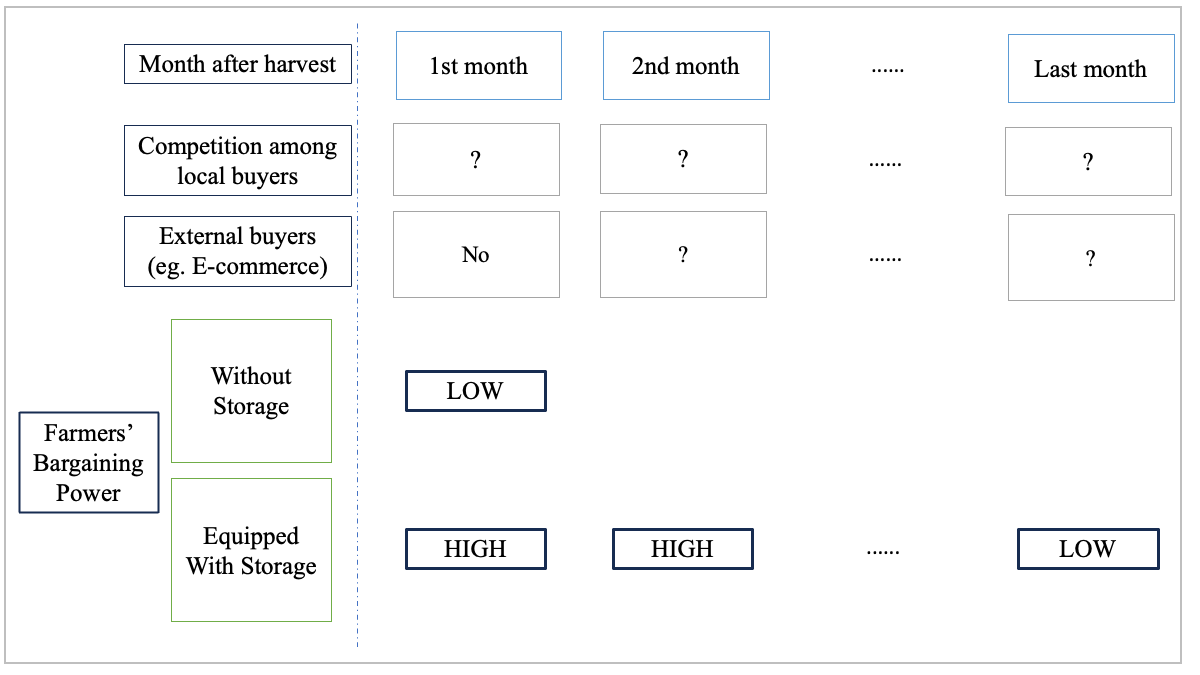
\includegraphics[width=1\textwidth]{figures/graphic_demo.png}
\caption{Extended Marketing Opportunities from Storage Adoption}
\label{Figure: Demo}
\end{figure}

Specifically, farmers could potentially benefit from increased competition in the oligopsonistic market through two sources. Firstly, the presence of different intermediaries in the village at various times can create fluctuating levels of competition on a monthly or even weekly basis. Secondly, farmers with storage can tap into additional distribution channels such as e-commerce and direct selling, which differ from the conventional middlemen-dominated system. By doing so, they can introduce external participants into the oligopsonistic market at the farm gate at different time nodes. 

I develop a conceptual framework to explore how smallholder farmers can adopt cold storage to potentially exploit the time-varying buyer power of middlemen. It considers a simplified dynamic, two-period scenario in a developing country, where farmers sell a specific cash crop to middlemen who visit local villages to procure the farm product. The model incorporates a storage-decision process, wherein farmers, observing farm-gate prices at harvest, decide whether to sell or store their crops.

The outcomes of this study hold substantial implications for policymakers and farmers alike. By exploring the dynamics of time-varying oligopsony levels, the research aims to demonstrate the potential benefits of storage facilities for smallholder producers. In a broader context, the findings suggest that embracing storage adoption could provide farmers with an effective alternative to combat anti-competitive practices like buyer collusion and market division and avoid more intrusive measures in markets, such as direct government intervention.





\section{Base Model}

I develop a two-period dynamic model to analyze how smallholder farmers strategically utilize storage in response to time-varying buyer power exerted by middlemen. The model is set in a rural area of a developing country, where farmers market a cash crop to itinerant traders. Harvest quantity is treated as exogenous, and the analysis focuses exclusively on farmers' storage and sales decisions within a single crop cycle. To identify the impact of market structure and trading dynamics, product quality is assumed homogeneous across farmers.

Farmers exhibit risk preferences ranging from risk neutrality to moderate risk aversion, valuing consumption at market prices. Each farmer is represented by a von Neumann–Morgenstern utility function,\footnote{An alternative mean-variance framework, presented in Appendix~\ref{Appendix: mean-variance approach}, yields similar insights. However, due to limited empirical guidance on calibrating the risk aversion coefficient within agricultural supply chains, the primary analysis relies on the utility-based framework.} $U_i(\pi_i)$, with $U_i' > 0$ and $U_i'' \leq 0$, where $\pi_i$ is the farmer's net income from crop sales. Farmers aim to maximize the expected utility of income across two trading periods.

The central decision is determining the proportion of the harvest stored immediately post-harvest, denoted by $s \in [0,1]$. This choice is made under uncertainty about future market conditions, specifically future buyer power dynamics in the subsequent trading period.

In the initial trading period, farmers observe farm-gate price offers from middlemen. Based on the frequency and dissemination of these offers, farmers infer the current buyer power, represented by $\theta_1$. Greater competition among buyers, characterized by lower $\theta_1$, correlates with higher farm-gate prices, $p_1$. Anticipating continuity in the inverse relationship between buyer power and prices across periods, farmers strategically allocate harvest between immediate sale and storage, incorporating expectations about future competition, captured by the random variable $\theta_2$.

Temporal demand variations downstream, such as seasonal shifts, are presumed fully anticipated by farmers and embedded into observed prices. Consequently, buyer power serves as the principal driver of intertemporal price variability in this model.

The model assumes symmetric information and negligible transaction costs in each trading period, ensuring farmers have complete and instantaneous access to prevailing farm-gate prices.

Formally, each farmer seeks to maximize expected utility over two trading periods by selecting storage share $s \in [0,1]$. Given a normalized harvest quantity $q = 1$, the optimization problem is:
\begin{equation}
\label{eq:starting objective}
\max_{s \in [0,1]} \mathbb{E} \left(U\left[ (1 - s) p_1 + s \cdot p_{2,\text{net}} \right]\right).
\end{equation}
where $p_1$ is the farm-gate price at harvest and $p_{2,\text{net}}$ is the second-period price adjusted for storage costs.



\subsection{Middlemen Market Structure and Farm-Gate Price Formation} \label{Section: Middlemen Market Structure and Farm-Gate Price Formation}
\noindent To analyze farmers’ strategic use of storage as a form of intertemporal bargaining, it is essential to model farm-gate price formation in a manner that flexibly incorporates the degree of competition among middlemen.

I adopt the \textit{Flexible Oligopoly/Oligopsony Market (FOOM)} framework to model farm-gate pricing as a function of buyer market power. Under the assumption that downstream markets, wholesale or retail, where traders sell the farm products they procure, are perfectly competitive, the farm-gate price $p_f$ is determined as:
\begin{equation}
p_f = \frac{p_r - mc}{1 + \frac{\theta}{\varepsilon}},
\end{equation}
where $p_r$ is the downstream price, $mc$ denotes the buyers’ constant marginal cost, $\theta$ captures the degree of buyer-side market power, and $\varepsilon$ represents the farm supply elasticity facing buyers.\footnote{For a detailed derivation, see Appendix~\ref{Appendix: Derivation of Farm Price under the FOOM Framework}.}


Normalizing the downstream price net of marginal cost to unity ($p_r - mc = 1$) for simplicity, the farm-gate price reduces to:
\begin{equation}
p_f = \frac{\varepsilon}{\varepsilon + \theta}.
\end{equation}


Although total harvest quantity is fixed at the time of the first-period decision, supply in that period remains somewhat elastic due to farmers’ ability to store part of their output. In period 2, supply is also elastic, as farmers can divert unsold produce to alternative buyers such as fruit-processing firms. To simplify the analysis while preserving these features, I assume a baseline supply elasticity of $\varepsilon_t = 1$ for both periods. This assumption serves as a plausible starting point and will be relaxed in subsequent analysis. Thus, farm-gate prices reduce further to:
\begin{equation}
p_f = \frac{1}{1+\theta}, \quad \theta \in [0,1],
\label{Eq: price formation by buyer power}
\end{equation}
where $\theta=0$ corresponds to perfect competition among buyers, $\theta=1$ reflects buyer monopsony or perfect collusion among buyers, and intermediate values capture varying degrees of oligopsony power.

Assuming farmers believe that this price formation rule persists across periods, period-specific prices are determined as $p_t = \frac{1}{1+\theta_t}, \quad t=1,2$. At harvest time, farmers observe $p_1$ and infer the contemporaneous buyer power, $\theta_1 = \frac{1 - p_1}{p_1}$. They then form expectations about the second-period buyer power, $\theta_2 \in [0,1]$, which is stochastic, and its distribution can be independent or based on the observation of $\theta_1$ under further assumptions. Thus, the second-period price can be expressed as:
\begin{equation}
p_2(\theta_2) = \frac{1}{1+\theta_2} 
\label{Eq: p_2 of buyer power change}
\end{equation}


To incorporate the economic cost of storage—including physical storage expenses, intertemporal discounting, and potential quality deterioration—I define the second-period price in net terms using a storage efficiency parameter $\kappa \in [0,1]$, which captures the overall storability of the commodity. Rather than modeling storage cost as a fixed deduction, I assume that storage frictions reduce the realized price proportionally, so that the farmer receives only a fraction $\kappa$ of the gross second-period price. This formulation captures a broad class of storage frictions, such as spoilage, shrinkage, and financing costs, that scale with the value of the commodity. It also reflects how farmers often perceive post-harvest losses: as a proportional reduction in potential revenue. From an analytical standpoint, the proportional specification preserves tractability under CRRA preferences, where utility is homogeneous of degree one and sensitive to relative rather than absolute changes in income. Accordingly, I define the net second-period price as:
$$
p_{2,\text{net}}(\theta_2) = \kappa \cdot p_2(\theta_2),
$$
where the gross second-period price remains $p_2(\theta_2) = \frac{1}{1 + \theta_2}$. Thus, the full expression becomes:
$$
p_{2,\text{net}}(\theta_2) = \frac{\kappa}{1 + \theta_2}.
$$
This setup ensures that the incentive to store responds coherently to economic fundamentals while allowing for an intuitive interpretation of $\kappa$: when $\kappa = 0$, the product is perfectly perishable and yields no second-period returns; when $\kappa = 1$, the product is perfectly storable with no loss in value—e.g., it can be left in a pile at the edge of the field.






\subsection{Final Objective Function}

\noindent Therefore, the economic environment at harvest could be summarized in Table~\ref{tab:baseline model parameter table}, capturing both observed and unobserved determinants of the farmer's storage decision over two periods.

\begin{table}[H]
\centering
\caption{Economic Environment at Harvest}
\label{tab:baseline model parameter table}
\begin{tabular}{lll}
\toprule
\textbf{Item} & \textbf{Symbol (units)} & \textbf{Status at Harvest} \\
\midrule
Harvest quantity & $q$ & Known, fixed (normalized to 1) \\
First-period price & $p_1$ & Observed \\
First-period buyer power & $\theta_1 = \frac{1 - p_1}{p_1}$ & Inferred from $p_1$ \\
Second-period buyer power & $\theta_2$ & Stochastic \\
Second-period price & $p_2 = \frac{1}{1 + \theta_2}$ & Derived \\
Storage efficiency factor & $\kappa \in [0,1]$ & Observed \\
Second-period net price & $p_{2,\text{net}} = \frac{\kappa}{1 + \theta_2}$ & Derived \\
CRRA risk aversion & $\gamma \in [0,1)$ & Observed \\
\bottomrule
\end{tabular}
\end{table}

\noindent The farmer allocates a share $s \in [0,1]$ of output to the second-period sale and retains the remainder for immediate sale at price $p_1$. Without a specific assumption on the utility functional form, substituting the expressions for $p_1$ and $p_{2,\text{net}}$, a farmer's maximization problem becomes:
\begin{equation}
\label{eq:final objective}
\max_{s \in [0,1]} \mathbb{E} \left\{U\left[\underbrace{\frac{1-s}{1+\theta_1}}_{\text{First-period income}} + \underbrace{s \cdot \frac{\kappa}{1+\theta_2}}_{\text{Adjusted second-period income}} \right]\right\}.
\end{equation}


\subsection{Risk Neutrality: Closed-Form Solution}
\noindent Under the case of risk neutrality, the utility function becomes linear: $U(\pi) = \pi$. The objective simplifies to:
\begin{equation}
\max_{s \in [0,1]} \; 
(1 - s) \cdot \frac{1}{1 + \theta_1} 
+ 
s \cdot \kappa \cdot \mathbb{E} \left[ \frac{1}{1 + \theta_2} \right].
\end{equation}
The solution simply depends on a comparison of marginal returns:
\begin{equation}
s^*( \gamma = 0) =
\begin{cases}
1 & \text{if } \kappa \cdot \mathbb{E} \left[ \frac{1}{1 + \theta_2} \right] > \frac{1}{1 + \theta_1}, \\
0 & \text{if } \kappa \cdot \mathbb{E} \left[ \frac{1}{1 + \theta_2} \right] < \frac{1}{1 + \theta_1}, \\
\text{any } s \in [0,1] & \text{if equality}.
\end{cases}
\label{Eq: risk-neutrality solution}
\end{equation}

\noindent Under risk neutrality, the farmer evaluates only expected monetary payoff. The decision reduces to a pure binary choice: if the net expected second-period price exceeds the normalized first-period price, then storage is optimal; otherwise, immediate sale dominates. Indifference arises only when the two expected returns are equal.


\subsection{Risk Aversion: Numerical Approach Needed}
\noindent In the presence of risk aversion—that is, when the utility function is strictly concave—analytical solutions to the farmer’s maximization problem are generally out of reach. This intractability arises from the fact that risk aversion embeds the random second--period buyer–power shock $\theta_2$ inside a nonlinear transformation.  With a strictly concave utility function $U(\cdot)$, the marginal utility term that enters the first-order condition is $U'\!\left[\frac{1-s}{1+\theta_1}+ s\frac{\kappa}{1+\theta_2}\right]$.  Because $s$ appears both outside and inside the expectation, the optimality condition requires solving
$$
\mathbb{E}\!\left\{\,U'\!\Bigl[\cdot\Bigr]\!\left[-\frac{1}{1+\theta_1}+\frac{\kappa}{1+\theta_2}\right]\right\}=0,
$$
which is a Fredholm integral equation. For generic concave $U$ (e.g., CRRA, CARA, or quadratic utility outside the linear range), the integral has no closed-form anti-derivative, because $U'$ must be evaluated at every realization of $\theta_2$ and then averaged over its distribution. Only by imposing knife-edge assumptions—such as risk neutrality ($U''=0$), degenerate $\theta_2$, or special affine-transform utility—does the expectation reduce to an algebraic expression that can be inverted for $s$.

Even when the distribution of $\theta_2$ is simple, analytic integration remains elusive. The ratio $\kappa/(1+\theta_2)$ introduces a hyperbolic term inside $U$, so the composition $U'\circ g(\theta_2)$ usually lacks a primitive.  Consequently, the derivative of the expected utility cannot be written as a finite combination of elementary functions, precluding a closed-form solution for the interior optimum. 

Moreover, risk aversion couples the mean and higher-order moments of $\theta_2$ through prudence.  The comparative-static effects of skewness or variance on $s^{*}$ therefore enter through higher-order derivatives of $U$, which are inseparable from the integral above.  This dependence further limits traceability.


These complications drive me to employ numerical analysis, specifically, the Monte Carlo evaluation of the expectation, to approximate the optimal storage share $s^{*}$ while respecting the corner constraints $s\in[0,1]$.





\section{Numerical Analysis} \label{Section: Base Model Numerical Analysis}
\noindent To examine how risk preferences and storage efficiency shape farmers’ intertemporal marketing decisions under buyer power uncertainty, I numerically solve for the optimal storage share $s^*$ across a range of parameter values. This section describes the simulation design and computational procedure employed to approximate the farmer’s decision problem under Constant Relative Risk Aversion (CRRA) utility.


\subsection{Setup and Parameterization}
\noindent A farmer is assumed to observe a moderate level of first-period buyer power $\theta_1 = 0.5$, the midpoint of the support. Second-period buyer power $\theta_2$ is stochastic and modeled using Beta distributions bounded on the unit interval $[0,1]$, allowing for flexible skewness and kurtosis while maintaining economically relevant support.

I consider eight distinct Beta distributions defined by a full factorial combination of:
\begin{itemize}
\item \textbf{Four means}: $\mu_{(\theta_2)} \in {0.2,,0.4,,0.5,,0.8}$, and
\item \textbf{Two variances}: $\sigma^2_{(\theta_2)} \in {0.02,,0.05}$, representing low and high uncertainty respectively.
\end{itemize}

For each $(\mu_{(\theta_2)}, \sigma^2_{(\theta_2)})$ pair, the corresponding shape parameters $(\alpha, \beta)$ are computed using the standard moment-matching formulas:

$$
\alpha = \mu_{(\theta_2)} \left( \frac{\mu_{(\theta_2)}(1 - \mu_{(\theta_2)})}{\sigma^2_{(\theta_2)}} - 1 \right), \quad
\beta = (1 - \mu_{(\theta_2)}) \left( \frac{\mu_{(\theta_2)}(1 - \mu_{(\theta_2)})}{\sigma^2_{(\theta_2)}} - 1 \right).
$$

I simulate 2,000 independent realizations of $\theta_2$ for each Beta distribution to approximate the expectation operator in the farmer's objective function.


\subsection{Simulation Grid}
\noindent The numerical analysis is conducted over the following two-dimensional grid:
\begin{itemize}
\item \textbf{Risk aversion}: $\gamma \in [0, 10]$, discretized over 30 evenly spaced points.
\item \textbf{Storage efficiency}: $\kappa \in [0.6, 1.0]$, discretized over 20 points.
\end{itemize}

This design spans a broad range of economically plausible values—from risk neutrality to strong risk aversion, and from low to perfect storage efficiency.

For each grid point $(\gamma, \kappa)$, I solve the farmer's problem by computing expected utility over a discrete set of 25 candidate storage shares $s \in [0, 1]$. The optimal share $s^*$ is the value that maximizes expected utility given the simulated distribution of $\theta_2$.


\subsection{Numerical Strategy}
\noindent The computational approach exploits a simplification under risk neutrality ($\gamma = 0$). In this case, the utility function becomes linear and the farmer's decision reduces to the binary rule as shown in Equation~\ref{Eq: risk-neutrality solution}.

For all $\gamma > 0$, I numerically evaluate a farmer's utility under the Constant Relative Risk Aversion (CRRA) functional form:
\begin{equation}
U(\pi)=\left\{\begin{array}{ll}
\frac{\left(\pi^{1-\gamma}-1\right)}{(1-\gamma)} & \text { if } \gamma \neq 1 \\
\ln (\pi) & \text { if } \gamma=1
\end{array},\right.
\label{eq: CRRA}
\end{equation}
where $\gamma$ denotes the coefficient of relative risk aversion, and $\pi$ represents the net income realized over two periods. 

The adoption of the Constant Relative Risk Aversion (CRRA) utility function is supported by both theoretical appeal and empirical evidence. Theoretically, CRRA maintains a constant degree of relative risk aversion across income levels, aligning with microeconomic models of choice under uncertainty. Empirically, panel data studies consistently find that the share of risky assets in household portfolios remains stable across wealth levels—even amid substantial income fluctuations—supporting the CRRA assumption \citep{Berger2020Characterizing, chiappori2011relative, zavala2024unfair}. The unitless nature of the CRRA coefficient $\gamma$ enables meaningful comparisons of risk preferences across settings and countries \citep{Szpiro1986Relative, hardaker2000some}. A recent meta-analysis by \citet{Irsova2025Relative} finds that, after adjusting for publication bias, the average coefficient of relative risk aversion centers around 1 in general economic applications and between 2 and 7 in financial contexts—figures that align closely with my field observations.




Moreover, this utility form aligns well with observed farmer behavior in regions proximate to my study sites. For example, \citet{jin2024losses} document persistent risk-averse decision-making among apple growers in areas that substantially overlap with the geographic scope of my fieldwork.

Each candidate $s$ is evaluated over the 2,000 simulated values of $\theta_2$, and the resulting utilities are averaged to approximate expected utility. The maximizer of this set yields $s^*$ for the given $(\gamma, \kappa)$ configuration.


\subsection{3D Visualization and Interpretation}
\noindent To present results, I construct a 4-by-4 panel as shown in Figure~\ref{Figure:3D_formulation}. The layout is organized as follows:
\begin{itemize}
\item \textbf{Top and bottom rows} plot the probability density functions (PDFs) of the eight Beta distributions used to simulate $\theta_2$. Each panel is annotated with its corresponding $(\mu_{(\theta_2)}, \sigma^2_{(\theta_2)})$ and the implied $(\alpha, \beta)$.
\item \textbf{Middle two rows} display 3D surfaces of the optimal storage share $s^*$ as a function of $\gamma$ and $\kappa$, separately for low-variance (second row) and high-variance (third row) distributions.
\end{itemize}
Each 3D plot is rendered with a consistent viewing angle such that the origin, corresponding to the lowest values of both $\gamma$ and $\kappa$, appears closest to the observer. These simulation surfaces depict key mechanisms driving intertemporal storage and marketing choices under local market-structural uncertainty in agriculture.

\begin{figure}[pht]
\centering
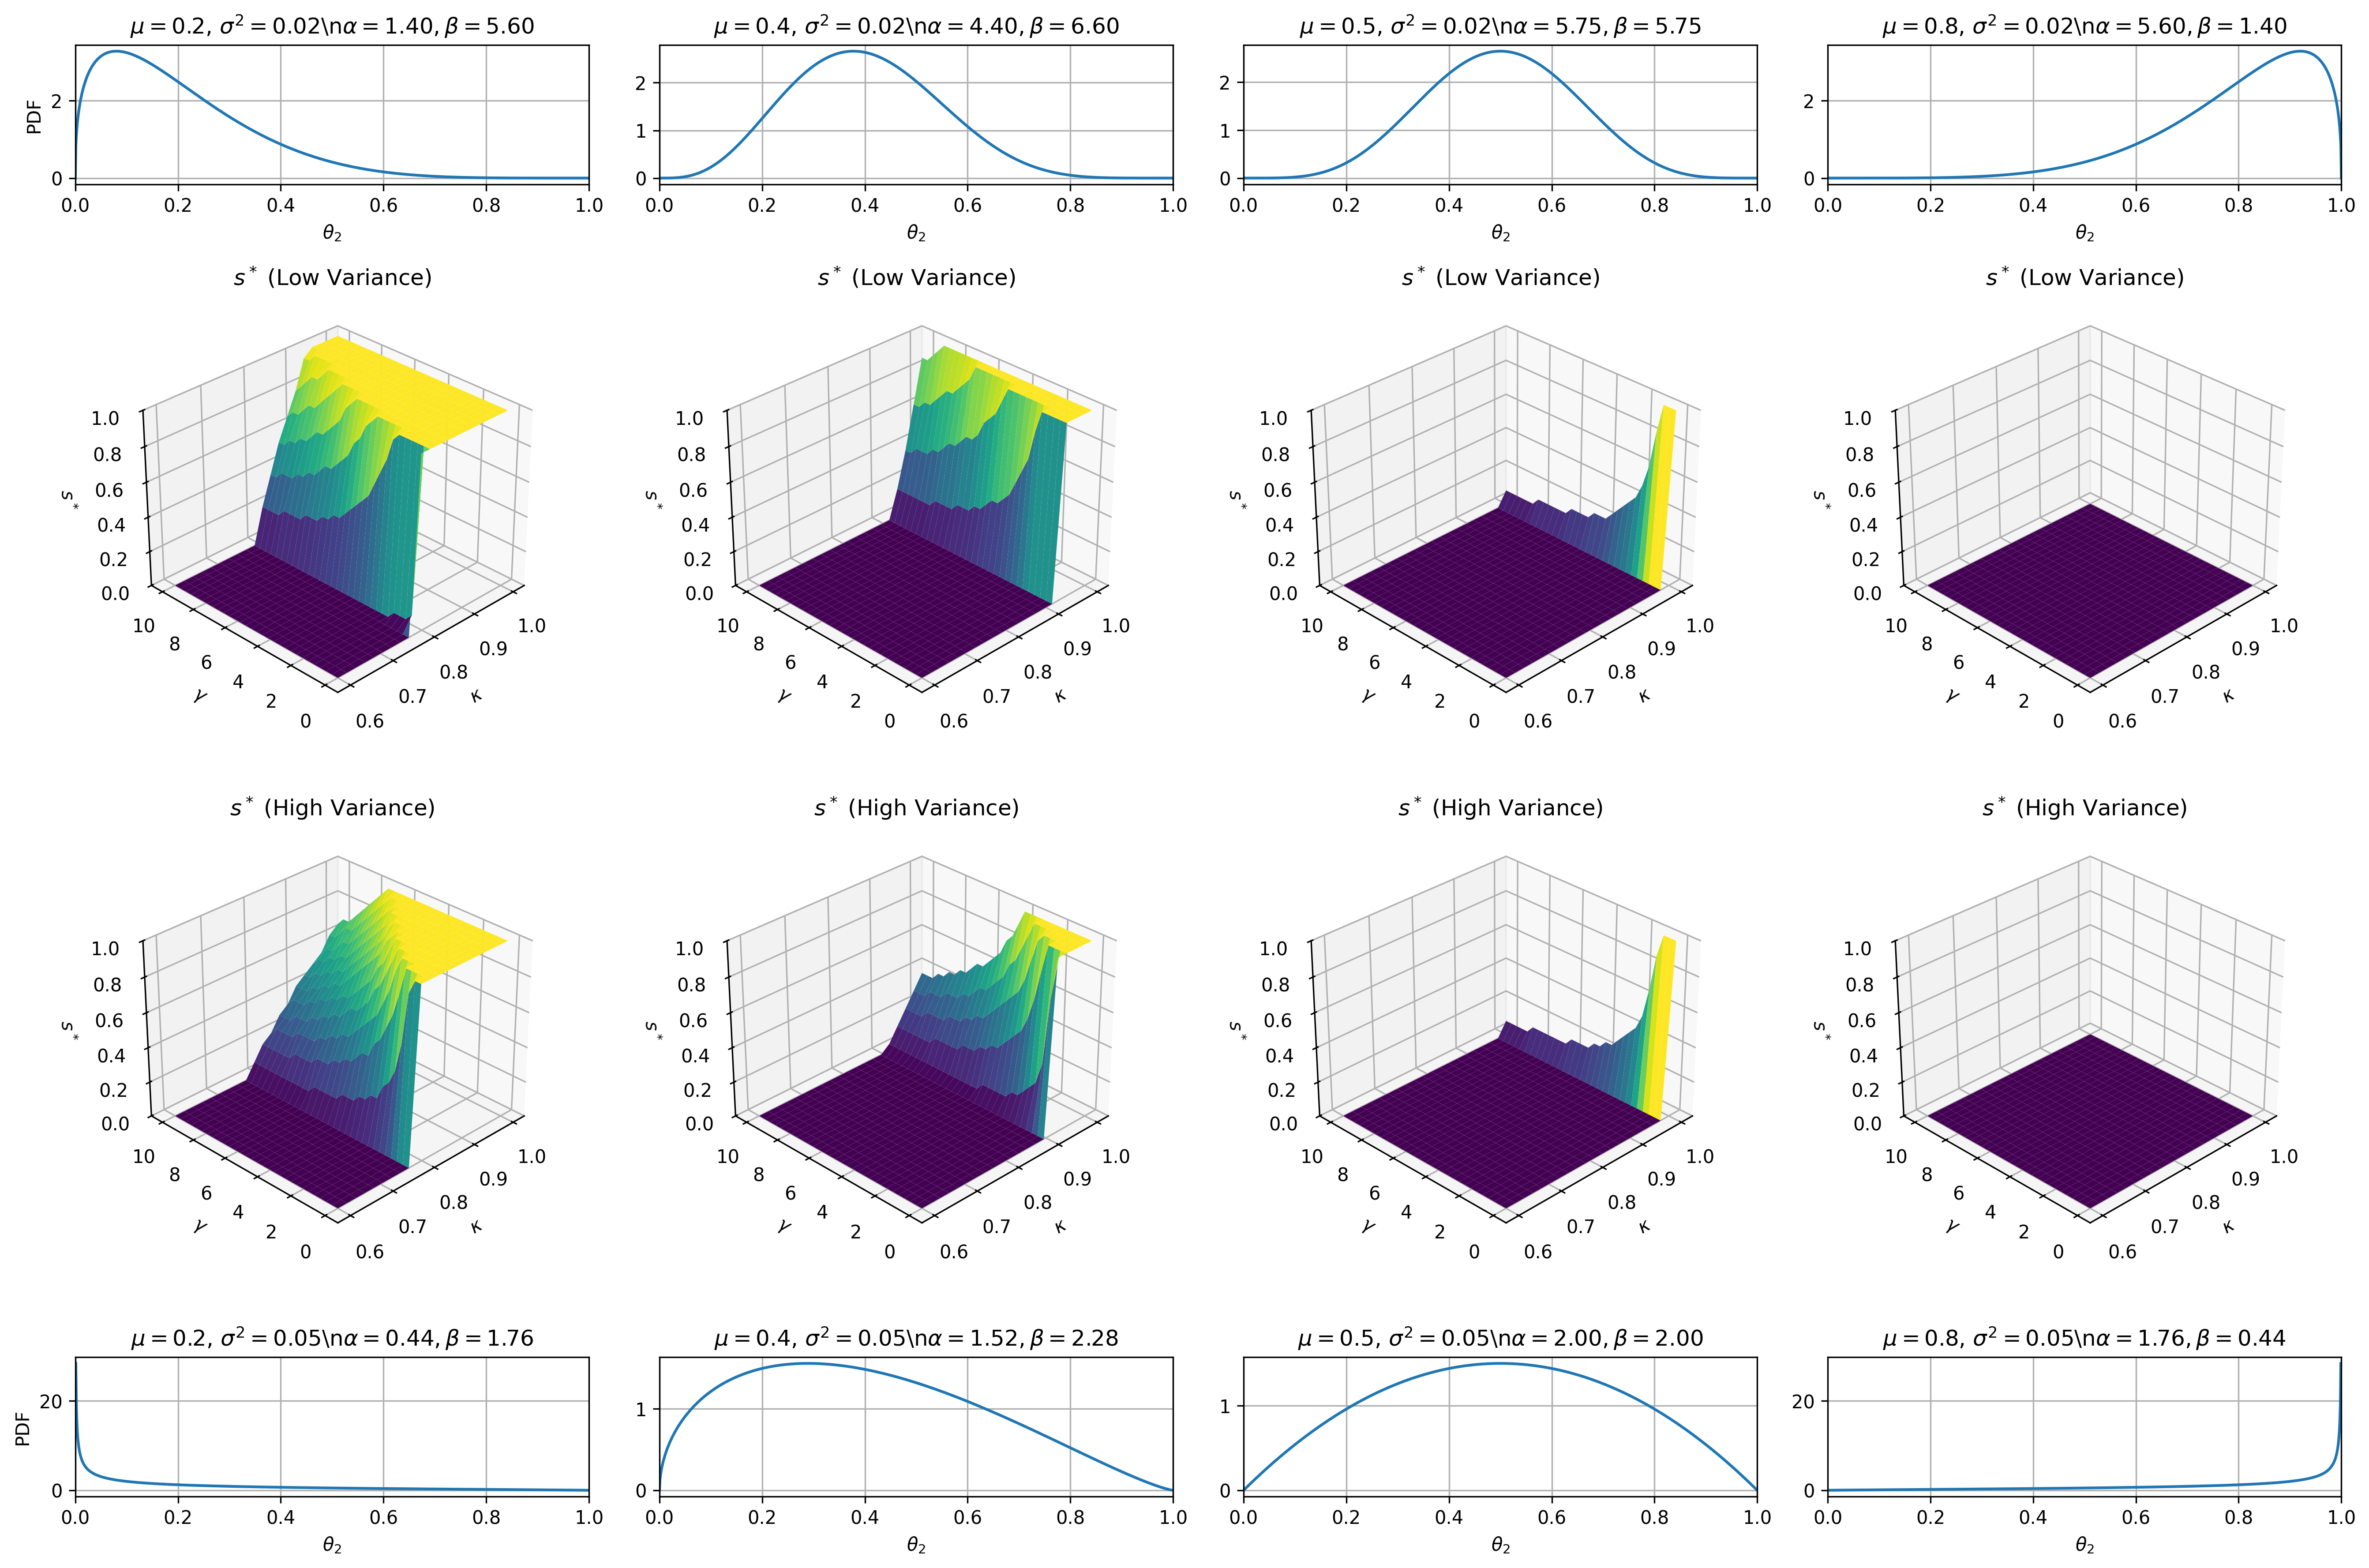
\includegraphics[width=\textwidth]{model_figures/3D_formulation.png}
\caption{Optimal Storage Share and PDF Visualizations under Eight Beta Distributions of $\theta_2$}
\label{Figure:3D_formulation}
\end{figure}

In general, when the farmer expects buyer power to be stronger in the future than at harvest—that is, when $\mathbb{E}[\theta_2] > \theta_1$—the incentive to store disappears. As illustrated in the far-right column of the panel, the optimal strategy across all risk and efficiency levels is to sell immediately ($s^* = 0$). In contrast, when expectations about future buyer power are neutral or favorable ($\mathbb{E}[\theta_2] \leq \theta_1$), the decision becomes more nuanced. Interior solutions ($0 < s^* < 1$) emerge over a meaningful range of risk preferences and storage efficiencies. Moreover, as the expected buyer power $\mathbb{E}[\theta_2]$ declines, both the scope for interior solutions and the frequency of corner solutions with full storage ($s^* = 1$) expand, reflecting the improved relative attractiveness of deferring sales.



Within each simulated surface, $s^*$ declines monotonically as $\gamma$ increases. This pattern is especially pronounced when future buyer power is moderate—that is, when expected second-period prices are only marginally higher than those in the first period. The underlying mechanism is intuitive: risk-averse farmers increasingly value certainty over potentially higher but uncertain future payoffs. As $\gamma$ rises, the disutility associated with price risk begins to outweigh the intertemporal arbitrage opportunity, especially when those gains are compressed by relatively high buyer power.



In contrast, storage efficiency $\kappa$ plays a reinforcing role. For a given level of risk aversion, increases in $\kappa$ make storage more attractive by reducing the effective cost of waiting. Accordingly, $s^*$ increases monotonically with $\kappa$, particularly when farmers are less risk-averse. The responsiveness of $s^*$ to $\kappa$ weakens at higher values of $\gamma$, suggesting that even highly efficient storage systems cannot fully offset the behavioral costs of risk exposure when farmers are strongly averse to uncertainty. 


Cross-panel comparisons further illustrate how changes in the distribution of second-period buyer power affect storage incentives. As the mean future buyer power $\mu_{(\theta_2)}$ increases (moving left to right across the panels), expected second-period prices decline, rendering storage less attractive in expected-value terms. Accordingly, the optimal storage share $s^*$ shifts downward across the entire surface. This effect is especially pronounced for risk-neutral or mildly risk-averse farmers, who condition decisions almost exclusively on expected returns. The lower the expected future price, the more immediate sale becomes the dominant strategy.



Variance in buyer power exerts a subtler influence. Comparing the second and third rows of the panel—low versus high variance cases—reveals that higher variance uniformly depresses $s^*$ across all parameter combinations. This effect reflects classical prudence: with concave utility, the marginal value of additional expected income diminishes in the presence of risk. Even when the expected second-period price remains high, increased dispersion in outcomes drives down the attractiveness of storage. The effect is pronounced at intermediate levels of $\gamma$, where farmers are sensitive to risk but not yet entirely averse to delayed selling.






\subsection{Sensitivity: Expected Future Buyer Power}
\noindent To further examine how a farmer’s optimal storage share $s^*$ responds to varying expectations about future buyer power, I conducted a simulation with the same parameter setting as in the 3D graphics above by holding first-period buyer power fixed at $\theta_1 = 0.5$, with a storage efficiency of $\kappa = 0.9$. The second-period buyer power $\theta_2$ was modeled as a Beta-distributed random variable with support on $[0, 1]$, maintaining a fixed variance of 0.02 while allowing the mean to vary from 0.05 to 0.95. For each mean value, I derived the associated Beta shape parameters and simulated 5,000 draws of $\theta_2$. The optimal storage share was then computed by maximizing expected utility under CRRA preferences, evaluated across five levels of risk aversion: $\gamma \in \{0, 0.5, 2, 4, 7\}$. As shown in Figure~\ref{Figure: sensitivity to second-period buyer power}, each resulting function $s^*(\mathbb{E}[\theta_2])$ was plotted to visualize how forward-looking uncertainty and risk preferences jointly shape storage behavior. Line color was varied monotonically with $\gamma$, increasing in darkness as risk aversion intensified.

The results reveal a distinct shift in behavior across risk preference levels. Under risk neutrality ($\gamma = 0$), the decision rule is binary: the farmer stores all output if the expected net-storage-cost second-period price exceeds the current one, and none otherwise. As $\gamma$ increases to positive values, the decision becomes more nuanced. The sharp threshold gradually turns into a smooth, decreasing function of $\mathbb{E}[\theta_2]$, with interior solutions appearing when the expected future buyer power is only marginally lower than the first-period one.


With higher risk aversion (like $\gamma = 4, 7$), the willingness to store declines substantially. Even when the expected second-period price exceeds today's price, the farmer often chooses to sell immediately due to the downside risk embedded in the distribution of $\theta_2$. The curve $s^*(\mathbb{E}[\theta_2])$ flattens near zero, and the turning point at which storage becomes attractive shifts leftward. This leftward shift reflects a heightened preference for certainty: more favorable expectations are required before any intertemporal transfer of output becomes worthwhile. 


\begin{figure}[pht]
\centering
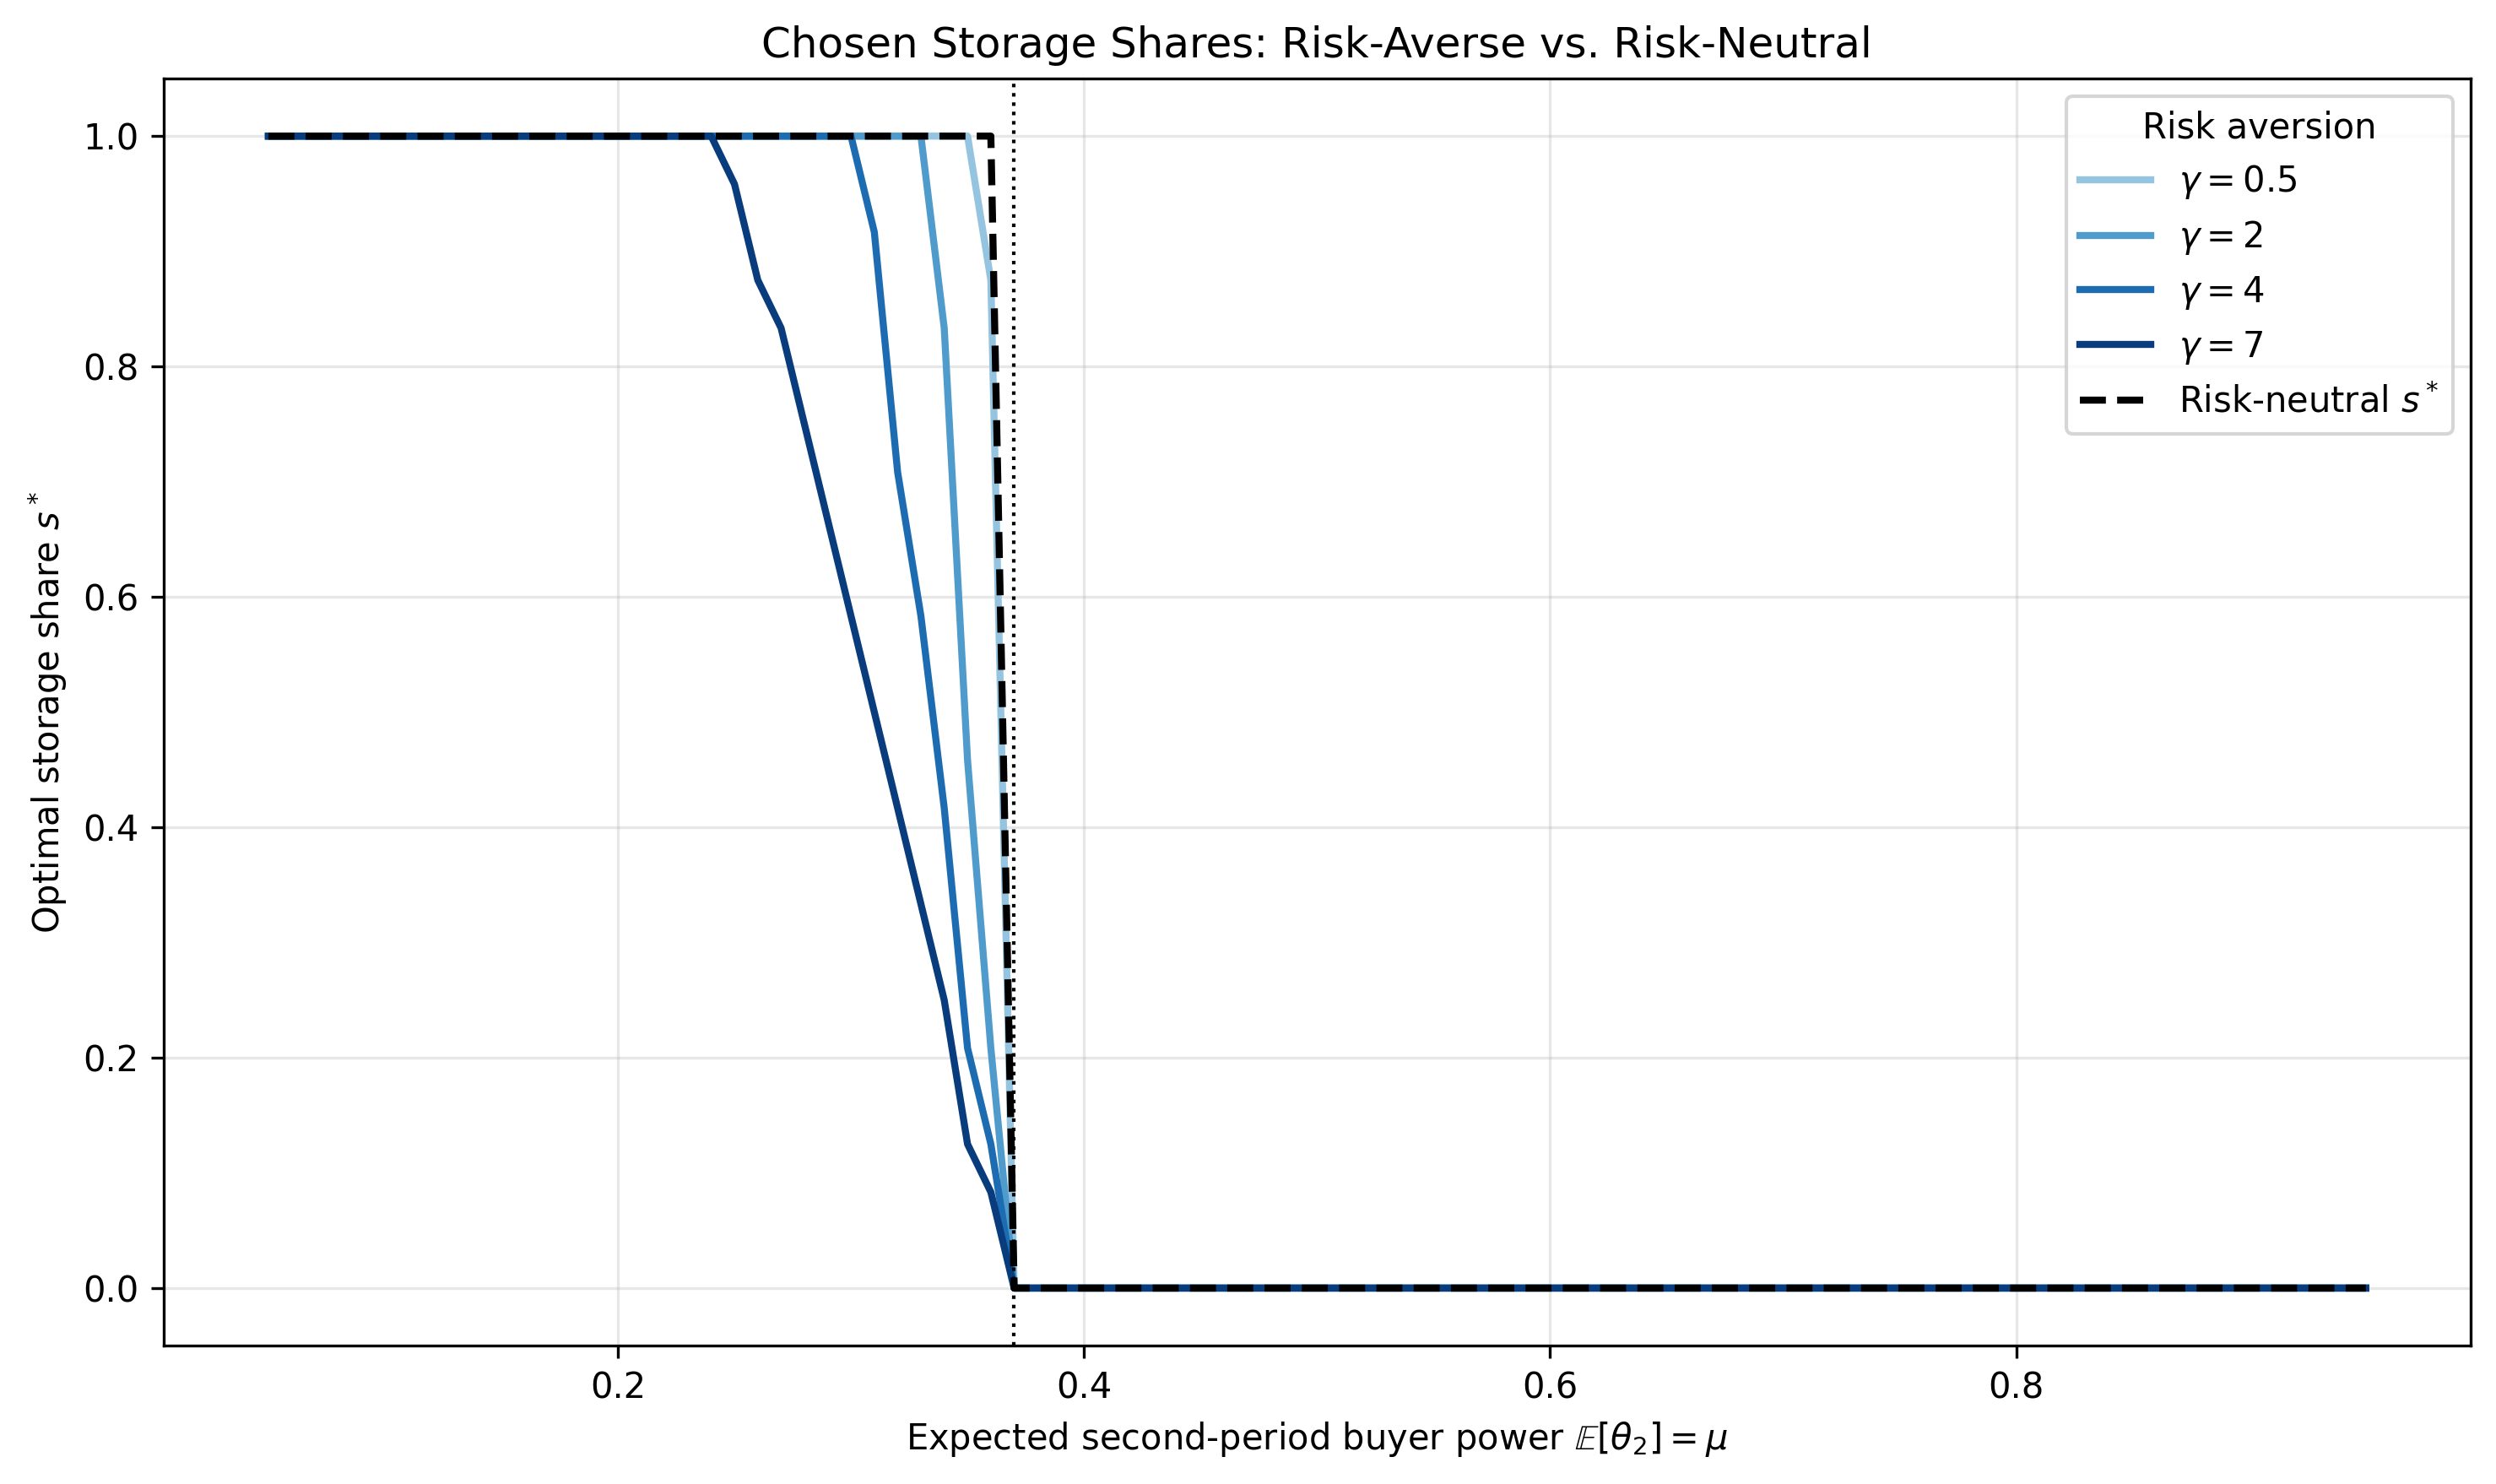
\includegraphics[width=\textwidth]{model_figures/sensitivity_to_theta_2.png}
\caption{Sensitivity to Expected Second-Period Buyer Power}
\label{Figure: sensitivity to second-period buyer power}
\end{figure}



\section{Special Cases: Explicit Competition Forms}
\noindent In the base framework above, buyer power is represented in a reduced-form manner of the \textit{FOOM} models through a nonlinear transformation into farm-gate prices. Specifically, buyer power $\theta$ was treated as an abstract, latent variable inferred from observed prices. To move beyond this generalized abstraction, I now discuss explicit models of non-cooperative buyer competition, excluding the consideration of buyer collusion, such as Bertrand (price-setting) and Cournot (quantity-setting) Competition. 

Suppose that instead of perceiving an unobservable level of buyer power, farmers observe the number of buyers present in the village at the time of harvest ($N_1$), and form expectations over the future one ($\mathbb{E}[N_2]$). The number of buyers in each period could range from one to a very large finite integer.

Bertrand and Cournot models represent distinct non-cooperative benchmarks for analyzing buyer competition. In the Bertrand framework, even a small number of buyers (as few as two) can lead to competitive outcomes with prices approaching marginal cost. In contrast, the Cournot model yields a more gradual relationship between the number of buyers and market outcomes, with prices converging to the competitive benchmark as buyer numbers increase.


\subsection{Bertrand Competition}
\noindent Under Bertrand competition, buyers set prices rather than quantities. If there are no capacity constraints, standard Bertrand logic implies that even two buyers suffice to drive the purchase price up to the competitive price, which is 1 under our derived price formation rule in Section~\ref{Section: Middlemen Market Structure and Farm-Gate Price Formation}. This phenomenon, known as the Bertrand Paradox, predicts perfectly competitive outcomes ($\theta_t=0$) as long as $N_t \geq 2$.

Therefore, under Bertrand conditions, according to Equation~\ref{Eq: price formation by buyer power}, the farm-gate price received by farmers can be modeled as:
\begin{equation}
p_t = 
\begin{cases}
0.5, & N_t = 1 \\
1, & N_t \geq 2
\end{cases}
\label{Eq: Bertrand Price Schedule}
\end{equation}
\noindent where $0.5$ denotes the monopsonistic reservation price paid when only one buyer is present. The transition from a single-buyer market to a multi-buyer market results in a discontinuous shift in price.

Here, I assume that farmers observe the first-period price at harvest, and the number of traders at a specific village in the second trading period ($N_2$) is stochastic, with the probability of one middleman being $\rho$, i.e., $Pr(n_2=1)=\rho$. So, the probability of multiple intermediaries appearing in village $j$ is $Pr(n_2 \geq 2) = 1-\rho$. \footnote{One possible explanation of the temporal difference in buyer presence is buyers' limited resources, such as an insufficient number of trucks to visit every village. Another factor could be collusion among traders, leading to the allocation of markets, turning each trader into a monopsony in their assigned markets during the designated periods \citep{herings2005intertemporal}. However, collusion is prone to breakdowns, as cartels are inherently unstable. Therefore, even if trader collusion occurs in period 1, it may not persist into period 2.}

Therefore, a farmer’s optimization problem in Equation~\ref{eq:final objective} could be written as follows:
\begin{equation}
\label{eq:Bertrand objective}
\max_{s \in [0,1]} \psi(\cdot) = \rho U((1-s)p_1 + \kappa s \cdot 0.5) + (1-\rho) U \left( (1-s)p_1 +  \kappa s \cdot 1 \right)
\end{equation}
where the first expression on the right-hand side reflects the utility from storing $s$ share of production to the second period in the monopsonistic case, and the second term represents the utility in the case of perfect competition among buyers.

Differentiating Equation~\ref{eq:Bertrand objective} with respect to $s$ gives the marginal utility gain from reallocating one unit of output from immediate sale to storage:

\begin{equation}
g(\cdot) = \frac{d\psi}{ds} = \rho U^{\prime}(\pi_L(s)) \cdot (-p_1 + \kappa \cdot 0.5) + (1 - \rho) U^{\prime}(\pi_H(s)) \cdot (-p_1 + \kappa)
\label{Eq: bertrand FOC}
\end{equation}
where $\pi_L(s) = (1 - s)p_1 + \kappa s \cdot 0.5$ and $\pi_H(s) = (1 - s)p_1 + \kappa s$ denote net income under low and high second-period prices, respectively.

Evaluated at $s = 0$—i.e., no storage—the marginal utility becomes:
$$
\left.\frac{d\psi}{ds}\right|_{s=0} = U^{\prime}(p_1) \cdot \left[\kappa(1 - 0.5\rho ) - p_1\right]
$$
The bracketed term reflects the expected net second-period price, net of storage loss. Since $U'(\cdot) > 0$, the sign of this expression determines whether storing is utility-improving. In particular, the farmer finds storage profitable ($s^* > 0$) if and only if:
$$
\kappa(1 - 0.5\rho) > p_1
$$
That is, expected gains from delayed sale, adjusted for storage inefficiency, must exceed the current price. If this inequality holds, deviating from zero storage increases expected utility. Then we can derive the following three lemmas:
\begin{lemma}
    The condition $\kappa (1 - 0.5\rho) < p_1$ is necessary and sufficient for the farmer to sell the entire harvest in the first period, $s^*=0$.
        \label{lemma: Bertrand no storage solution}
\end{lemma}
\begin{proof}
    From Equation~\ref{Eq: bertrand FOC}, we can derive the second-order condition $\frac{d^2 \psi}{d s^2} = \rho U^{\prime \prime}\left(\pi_L(s)\right) \cdot\left(-p_1+ \kappa \cdot 0.5\right)^2+(1-\rho) U^{\prime \prime}\left(\pi_H(s)\right) \cdot\left(-p_1+\kappa\right)^2$. Since $U^{\prime\prime}(\cdot)\leq0$, the entire RHS expression is non-positive. Therefore, when $\kappa (1-0.5\rho) < p_1 $, the $\frac{d \psi(s=0)}{d s}$ would never be positive.
\end{proof}


\begin{lemma}
    On the contrary, when $\kappa (1-0.5\rho) > p_1 $ and $\frac{d \psi(s=1)}{d s}>0$, then the farmer maximizes utility by storing the entire harvest for second-period sale, $s^*=1$.
    \label{lemma: Bertrand full storage solution}
\end{lemma}
\begin{proof}
    As $\kappa (1-0.5\rho) > p_1 $ secures a positive storage share proven above, $\frac{d \psi(s=1)}{d s}>0$ ensures that expected utility is increasing in $s$. Therefore, at any given point of $s$, it would be optimal for the farmer to store more to get higher utility till $s$ reaches its upper bound.
\end{proof}


\begin{lemma}
    A farmer optimally adopts partial storage strategy (i.e., marketing production through both periods, $s^*\in (0,1)$) when the conditions $g(\cdot)  =  \frac{d \psi}{d s} = 0$ and $g^\prime(\cdot) = \frac{d^2 \psi}{d s^2} < 0 $ (implying a strictly risk-averse farmer), are satisfied in the range $0<s<1$.
    \label{lemma: Bertrand Interior solution}
\end{lemma}
\begin{proof}
    This is a standard interior optimum: the first-order condition holds and the second-order condition ensures a local maximum. Strict risk aversion ($U^{\prime\prime} < 0$) guarantees concavity and uniqueness.
\end{proof}

These three lemmas establish a complete characterization of the farmer’s storage behavior: sell immediately, store fully, or split output across periods. Because the first-period price $p_1$ is itself endogenously determined by buyer competition (Equation~\ref{Eq: Bertrand Price Schedule}), we examine two benchmark cases: $p_1 = 1$ and $p_1 = 0.5$.

When multiple buyers are present at harvest, Bertrand competition drives the price to its competitive level, $p_1 = 1$. In this case, the expected second-period price, $\kappa(1 - 0.5\rho)$, falls below $p_1$, implying—by Lemma~\ref{lemma: Bertrand no storage solution}—that the farmer optimally sells all output immediately ($s^* = 0$). The benefit of immediate competition dominates any incentive to store.

In contrast, under monopsony at harvest ($p_1 = 0.5$), the storage incentive becomes ambiguous. The net gain from storing simplifies to $(\kappa -0.5)(1 - \rho)$, which is positive as long as: (i) the competitive price, adjusted for storage loss, exceeds the monopsonistic price; and (ii) there is a nonzero probability of facing competitive pricing in the second period ($\rho < 1$). Under these conditions, both full storage and interior storage solutions are feasible, depending on the form of risk aversion and specific parameter values.

Under monopsonistic first-period pricing, local comparative statics can be derived using the implicit function theorem. Let $g(s) = \frac{d\psi}{ds}$ denote the first-order condition for interior optimality. Then for any parameter $\xi \in {\rho, \kappa, p_1}$, the sensitivity of the optimal storage share satisfies:
$$
\frac{\partial s^*}{\partial \xi}= -\frac{\frac{\partial g}{\partial \xi}}{\frac{\partial g}{\partial s}}
$$
Since the second-order condition ensures $\partial g / \partial s = \frac{d^2\psi}{ds^2} < 0$, the sign of $\frac{\partial s^*}{\partial \xi}$ is governed by the sign of $\partial g / \partial \xi$. However, with the exception of the storage efficiency factor $\kappa$—where lower storage cost unambiguously increases storage—the comparative statics with respect to $\rho$ and $\kappa$ are not signed deterministically. This limits the interpretive power of local sensitivity analysis, especially given the narrow parameter region where an interior solution $s^* \in (0,1)$ arises, as shown in the previous section.







\subsection{Cournot Competition}
\noindent In contrast, under Cournot competition, each buyer chooses the quantity to purchase simultaneously, assuming that other buyers’ quantities are fixed. The resulting equilibrium reflects strategic quantity-setting behavior. In this setup, price is no longer polarized, but a smoother function of the number of active buyers.

Given this relationship, and maintaining the same linear demand structure used in Section~\ref{Section: Middlemen Market Structure and Farm-Gate Price Formation}, the resulting equilibrium price in each period $t$ under Cournot competition is:
\begin{equation}
    p_t = \frac{N_t}{N_t + 1}, \quad t = 1,2.
\end{equation}
where $N_t$ is within the range of non-negative integers, and hence the bound of $p_t$ is $[0, 1)$. This expression captures the inverse relation between market structure conditions and farm-gate prices: as $N_t$ increases, buyer power declines, and the price approaches the competitive limit of 1. Conversely, when $N_t$ is small, buyer power is significant, and prices are suppressed. When no one comes to a village, i.e., $N_t=0$, it leads to market failure. 

Therefore, a farmer's maximization problem under the case of Cournot competition would be highly similar to Equation~\ref{eq:final objective} in the base model, but with a different farm-gate price formation rule:
\begin{equation}
\label{eq:Cournot objective function}
\max_{s \in [0,1]} \mathbb{E} \left\{U\left[\underbrace{\frac{(1-s)N_1}{1+N_1}}_{\text{First-period income}} + \underbrace{ s \cdot \kappa \cdot \frac{N_2}{1+N_2}}_{\text{Adjusted second-period income}} \right]\right\}
\end{equation}
where $N_1$ is observed at harvest and $N_2$ is a stochastic element. To solve this maximization problem, a numerical simulation is needed.


Let's model the second-period buyer count $N_2$ as a discrete Poisson-distributed random variable truncated to the interval $[0,9]$, capturing uncertainty in buyer presence.  I fix storage efficiency at $\kappa = 0.9$ and first-period buyer count at $N_1 = 3$ as the baseline.\footnote{I set $N_1=3$ here because in my fieldwork surveys, the mean of first-period buyer count is 3.34 and the median is 3.} As in Section~\ref{Section: Base Model Numerical Analysis}, farmers are assumed to have constant relative risk aversion (CRRA) preferences.

Four different Poisson means, $\mu \in \{8, 4, 3, 1\}$, are considered, each representing different expectations about second-period market thickness. For each case, I simulated 5,000 realizations of $N_2$ and constructed a 2×4 panel plot in Figure~\ref{Fig: 3D Cournot}. The top row of the panel displays the probability mass functions (PMFs) of the Poisson distributions, offering a visual representation of how buyer count uncertainty is distributed under each mean. The bottom row presents 3D surface plots of the optimal storage share $s^*$ as a function of risk aversion $\gamma \in [0,10]$ and storage efficiency $\kappa \in [0.6, 1.0]$ as our baseline model. The CRRA utility framework was applied, and a closed-form solution was used when $\gamma = 0$. The results show that $s^*$ increases with both higher storage efficiency and lower risk aversion. Moreover, when the expected number of second-period buyers is low (e.g., $\mu = 1$), farmers optimally store less—particularly if they are risk averse—due to the weak and uncertain market prospects.

\begin{figure}[htp]
    \centering
    \begin{subfigure}{\textwidth}
        \centering
        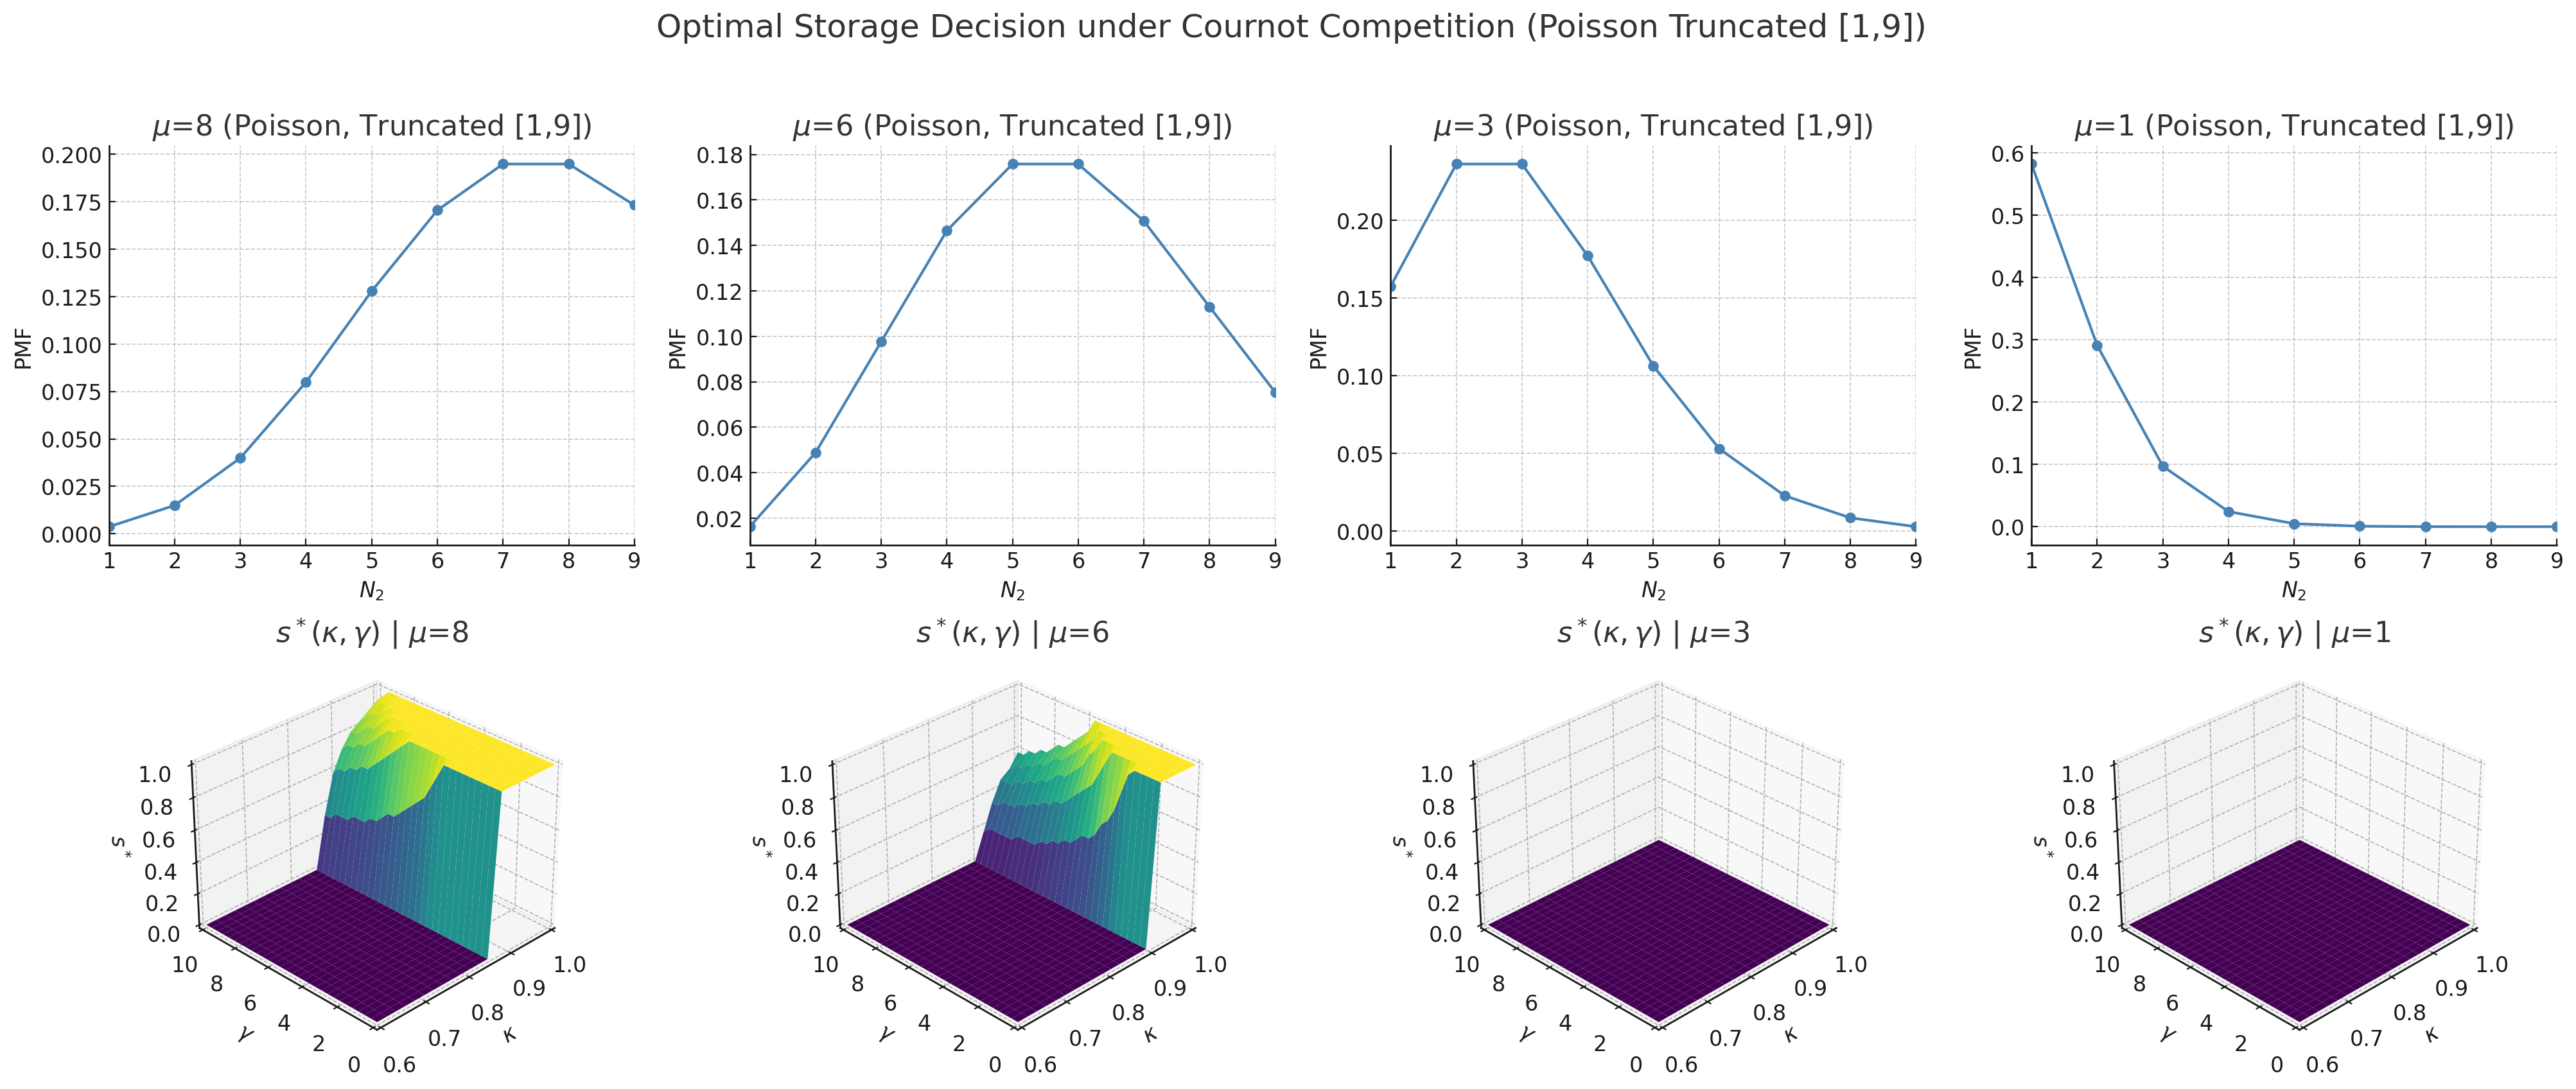
\includegraphics[width=\textwidth, keepaspectratio=true]{model_figures/3D_cournot.png}
        \caption{Optimal Storage Share and PDF Visualizations under Four Poisson Distributions of $N_2$}
        \label{Fig: 3D Cournot}
    \end{subfigure}
    
    \vspace{10mm} % Reduced vertical gap between subfigures
    
    \begin{subfigure}{\textwidth}
        \centering
        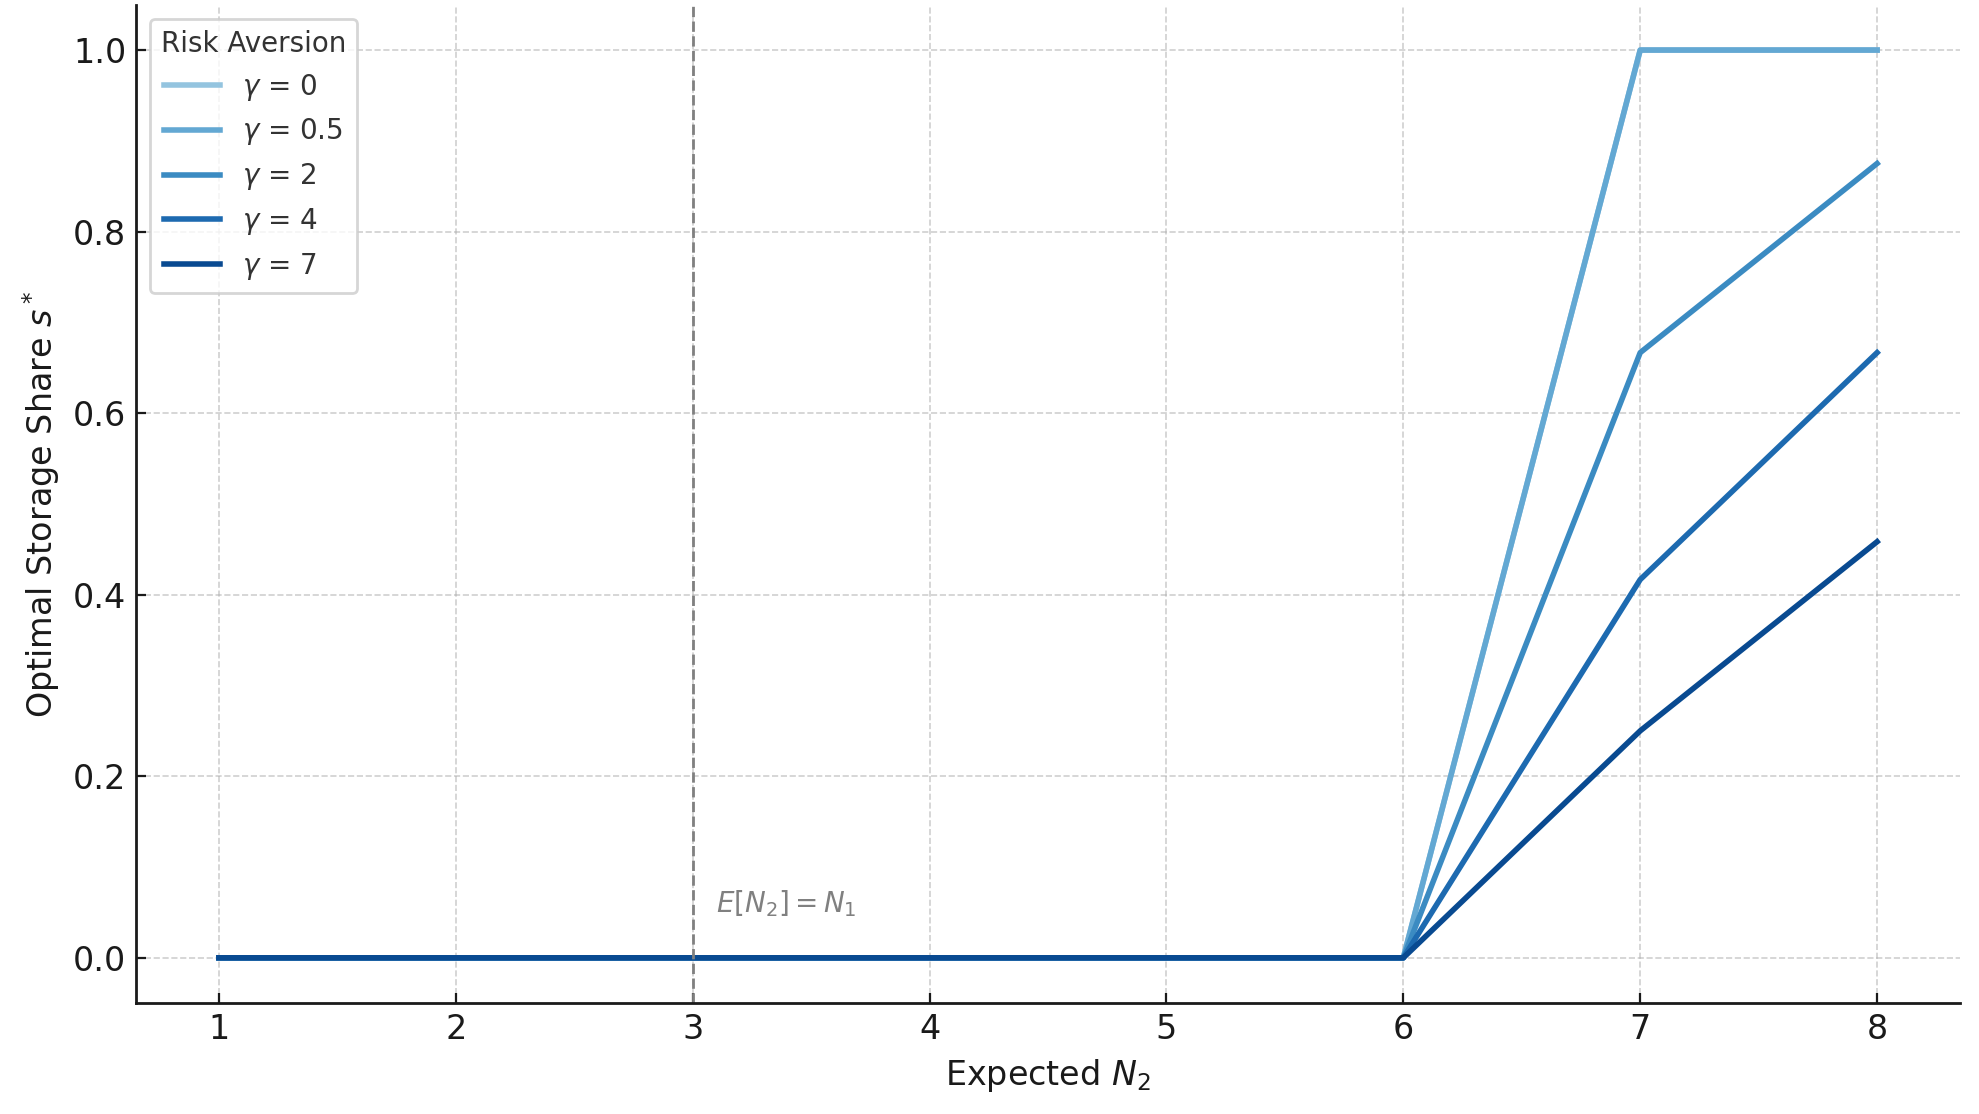
\includegraphics[width=\textwidth, keepaspectratio=true]{model_figures/buyer_count_sensitivity_cournot.png}
        \caption{Sensitivity to Expected Second-Period Buyer Presence}
        \label{Fig: Cournot sensitivity}
    \end{subfigure}

    \caption{Numerical Analysis under Cournot Competition}
\end{figure}

To further explore the effects of expectations about second-period buyer power under different levels of risk aversion, I varied the expected second-period buyer count $\mathbb{E}[N_2]$ from 1 to 8 in increments of 1 by simulating truncated Poisson distributions. For each expected value, I computed the farmer’s optimal storage share $s^*$ under five levels of risk aversion: $\gamma \in \{0, 0.5, 2, 4, 7\}$.

The resulting line plot in Figure~\ref{Fig: Cournot sensitivity} overlays the five curves of $s^*(\mathbb{E}[N_2])$, each representing a different risk aversion level. To visually distinguish them, darker lines correspond to higher risk aversion. A vertical dashed line is added at $\mathbb{E}[N_2] = N_1$ to indicate the benchmark where both periods have symmetric market conditions. For all $\gamma$, $s^*$ increases as the expected second-period buyer count rises, reflecting improving market prospects. More risk-averse farmers (higher $\gamma$) are generally less willing to store unless second-period conditions are significantly better than the present.

A key insight is that even under a low composite storage cost ($\kappa=0.9$) and a relatively competitive market structure at harvest ($N_1=3$), farmers would consider storage as an option only when the expected number of buyers visiting during the second period is at least doubled ($\mathbb{E}[N_2]\geq 6$), which is a direct result from the Jensen's Inequality when we derive the expectation of second-period price. In other words, only a very strong optimistic expectation of future buyer presence would lead a farmer to use storage to arbitrage across two periods, even for those risk-neutral farmers. 





\subsection{Connected to Fieldwork}



\begin{figure}[hpt]
\centering
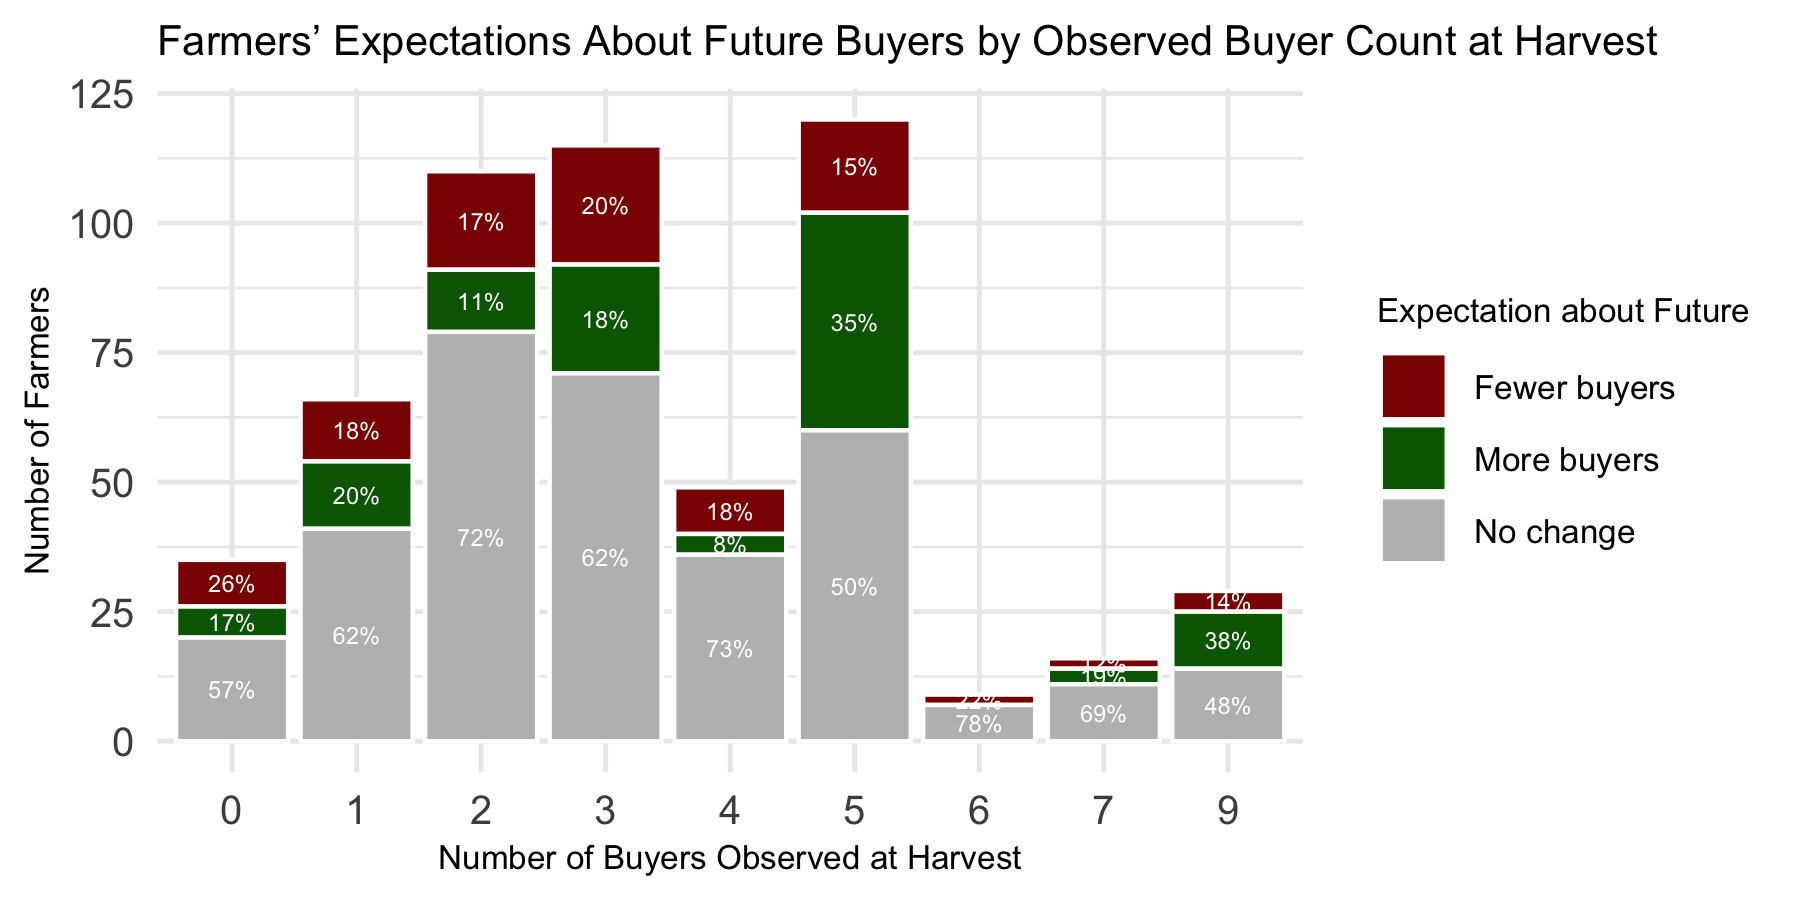
\includegraphics[width=\textwidth]{figures/buyer_count_distribution.png}
\caption{Observed Buyer Count at Harvest with Farmers’ Expectations About Future Buyers}
\label{Figure: buyer count at harvest}
\end{figure}





%----------------------------------------------------%
%----------------------------------------------------%


\section{Further Extensions}

\subsection{Other Models of Risk Preference}
\noindent According to \cite{o2018modeling}, "Real-world risk aversion is clearly not as straightforward as expected utility suggests. Additional sources of risk aversion (or risk-seeking) need to be used instead of, or in conjunction with, diminishing marginal utility of wealth." Individuals assess options involving both gains and losses, the "kink" in the value function between losses and gains induces risk aversion. Therefore, future researchers may extend my model by exploring the Loss Aversion models \citep{kahneman1979prospect}, in addition to the expected utility theorem. The approach developed by \cite{kHoszegi2006model, kHoszegi2007reference, kHoszegi2009reference} in addressing loss aversion with an endogenous reference point aims to mitigate this degree of freedom by asserting that the reference point is entirely determined by one's expectations about outcomes. Despite this, there has been limited progress in adapting alternative models to dynamic settings, with a notable exception of \cite{kHoszegi2009reference}, who define loss aversion concerning changes in beliefs regarding both current and future consumption.



\subsection{Collective-Action Dilemma: Storage "Treadmill"}
\noindent Another important observation from the fieldwork is that increasing storage adoption among farmers in a village may discourage buyers from visiting there. If the majority of farmers in a village adopt storage, middlemen may redirect their focus to other villages where farmers have not yet embraced this technology. This spillover effect could stem from middlemen favoring farmers with less bargaining power, as they could negotiate lower prices for the crops they purchase. This leaves farmers without storage in this well-equipped village facing less competitive market conditions and creates in essence an escalating incentive within the village to obtain storage. However, the higher the adoption rate in this village, the lower the marginal benefit of storage adoption is as the less likely the traders would visit there. Therefore, this creates a storage "treadmill" similar to the technology treadmill envisioned by Willard Cochrane \citep{levins1996treadmill, cochrane1958farm}. Further analysis could discuss this collective-action dilemma and try to introduce a parameter into the current model to capture it.


\subsection{Non-linear Storage Cost}
\noindent Storage costs for farmers, defined as the sum of the actual cost of renting or operating storage space and the cost of deterioration, could be non-linear in many cases. For perishable goods like apples, the primary reason for convex storage costs is probably that spoilage and quality deterioration increase over time. Also, the operating costs of storage may not increase linearly with the volume of goods stored. Managing temperature and humidity conditions for larger quantities might require more sophisticated technology and energy consumption, leading to non-linear cost increases.

Supporting this notion, \cite{williams1989economic} demonstrates, through a quadratic form of total marketing costs, that farmers need to weigh the marginal revenue of later sales against the elevated costs incurred. This balance leads to a positive inventory, even without considering risk aversion. Instead of capturing the composite storage cost by a discounting factor, a well-designed mathematical model would allow other forms of storage costs, therefore, may give us other relevant real-world policy implications.



\section{Conclusion}
\noindent This chapter demonstrates that storage adoption can have a dynamic impact on the welfare of farmers facing oligopsony power, providing inter-temporal arbitrage opportunities and stronger bargaining power over time. Cold storage adoption helps farmers overcome trading-time limitations and benefit even from temporal changes in trader competition alone. Examining storage from a market competition perspective offers a fresh approach to analyzing the influence of inventory on growers' and sellers' marketing strategies and their bargaining power.

My baseline model provides a theoretical basis for small-scale farmers' storage and marketing choices in developing countries. It focuses on farmers' intra-seasonal strategies and the storing-decision process, where farmers observe farm-gate prices and market structure at harvest and decide whether to immediately sell some, all, or none of their crops. When farmers have insufficient bargaining power at a single point in time, the adoption of storage at lower storage costs would give them inter-temporal arbitrage opportunities. 

Therefore, in many developing countries, government policies can replace or supplement the existing minimum purchase price and direct cash transfers by subsidizing farmers' investment in storage infrastructure. Instead of intervening directly in markets by using quality-preserving technology broadly to sell their harvest at an optimal time, the government can empower farmers to gain stronger bargaining power against middlemen and benefit both consumers and growers in the agricultural industry supply chains.

This chapter's application extends beyond the fresh apple industry to various settings. Cold storage and inventory play a crucial role in transactions, commonly seen as tools to help sellers take advantage of business cycle fluctuations. However, the competitive dynamics among buyers can vary over time, even without changes in demand or supply elsewhere in the industry chain. By examining storage from a market competition perspective, this model offers a fresh approach to analyzing the influence of inventory on growers' and sellers' marketing strategies and their bargaining powers in agricultural commodity industries.




% %---------------------------%
% \newpage
% \section{Memo: A Difficult Tradeoff between Two Utility Aggregation Approaches}
% \noindent As I finalize revisions on the current model, I identify a major conceptual drawback: the optimal storage share becomes increasing in the farmer’s degree of risk aversion when the expected second-period buyer power is higher than the first-period level. In other words, the model implies that farmers who expect a worse market condition in the future would store more if they are more risk-averse. This result is counterintuitive and lacks a clear behavioral or economic justification.

% This inconsistency has prompted me to revisit an alternative formulation we previously considered. Specifically, we face a fundamental modeling choice between:
% \begin{itemize}
%     \item Maximizing the expected sum of discounted utilities of income, versus
%     \item Maximizing the utility of the sum of discounted incomes.
% \end{itemize}
% Both approaches are theoretically sound but carry distinct implications. Below, I outline the tradeoffs between the two so we can more clearly evaluate the direction forward.

% \subsection{Current Setting: Sum of Discounted Utilities of Income}

% \noindent This is the standard formulation in intertemporal utility theory, where utility is evaluated separately in each period and future utility is discounted by a factor $\delta$:
% \begin{equation}
% \max_{s \in [0,1]} ; U\left((1 - s) p_1\right) + \delta \cdot \mathbb{E} \left[ U\left(s \cdot p_{2,\text{net}} \right) \right].
% \end{equation}

% \noindent Key assumptions and implications:
% \begin{itemize}
% \item Utility is additive and separable across time.
% \item The agent is risk-averse within each period, but not across periods.
% \item This structure implies a preference for income smoothing over time.
% \end{itemize}

% The primary advantage of this formulation lies in its analytical tractability. The separability allows us to derive a closed-form solution for the optimal storage share $s^*$, even under nontrivial distributional assumptions about future buyer power. It fits neatly within the expected utility framework and supports comparative statics analysis with intuitive results, except for the key case of higher second-period buyer power involving risk aversion.

% Through simulation and sensitivity checks (see Figure), I observe a troubling result: when expected second-period buyer power is pessimistic ($\theta_2$ is larger), the optimal storage share becomes increasing in risk aversion. This is counterintuitive. Typically, greater risk aversion should lead agents to reduce exposure to future uncertainty—i.e., store less. This expected behavior holds in the left region of the figure (where expectations about the future are optimistic), but breaks down in the right region.

% Upon closer inspection, this anomaly stems from the fact that the model assumes risk aversion only within periods. The framework lacks intertemporal risk aversion—i.e., there is no mechanism to penalize uncertainty in total income across periods. Unless we fundamentally alter the utility function (e.g., by adopting a non-additive or piecewise utility structure), this counterintuitive outcome cannot be avoided within this setting.

% One might ask how prior literature addresses this. The answer is: they often avoid it by making restrictive assumptions or narrowing the scope of analysis. For instance, \citet{ruhinduka2020smallholder} (the work by Travis Lybbert and his co-authors studying the post-harvest storage decisions) assume $\mathbb{E}(p_2) > p_1$, ensuring that $\partial s^* / \partial \gamma < 0$, thus sidestepping the unintuitive regime altogether.


% \subsection{Alternative Setting: Utility of the Sum of Discounted Income}
% \noindent This alternative formulation, similar to the structure used in your work with Saitone and Malan \citep{saitone2018price}, applies the utility function to the entire stream of income, aggregated and discounted to the present:
% \begin{equation}
% \max_{s \in [0,1]} ;\mathbb{E} \left(U\left[ (1 - s) p_1 + \delta \cdot s \cdot p_{2,\text{net}} \right]\right).
% \end{equation}

% \noindent Key assumptions and implications:
% \begin{itemize}
% \item Utility is applied to the total discounted income as a single aggregated payoff.
% \item The agent exhibits intertemporal risk aversion—preferences depend on risk in the total income stream, not just within each period.
% \item This formulation is commonly used in investment and project evaluation models, especially under uncertainty.
% \end{itemize}

% The primary strength of this setting is its consistency with empirical observations. Simulations under a CRRA utility specification (see Figure show that both risk-neutral and most moderately risk-averse farmers tend to make corner solutions—either storing everything or nothing—which aligns well with real-world behavior. Interior solutions exist but are confined to a narrow region of the parameter space, unlike the smoother, wider range of partial storage outcomes generated by the standard model.

% The main limitation, however, is analytical intractability. Closed-form solutions for the optimal storage share $s^*$ are not available under arbitrary distributions of $\theta_2$ in our case. Solving this model typically requires numerical methods, which restrict our ability to conduct formal comparative statics. An exception arises in cases with a finite number of discrete scenarios—e.g., buyer competition modeled as Bertrand duopoly with known probabilities—in which case closed-form solutions may be derived. Otherwise, we must rely on simulation-based approximation.

% \subsection{3D Visualizations of Both Formulations}

% \noindent I conduct simulations for both utility formulations over a grid defined by the coefficient of relative risk aversion ($\gamma$) and the storage efficiency factor ($\kappa$). The first-period buyer power is fixed at $\theta_1 = 0.6$, and the discount factor is set at $\delta = 1.0$ throughout.

% Figure~\ref{fig:3D_formulation} presents a $4 \times 4$ panel summarizing the simulation results. I examine eight distinct Beta distributions for $\theta_2$, varying in both the mean and variance: two levels of variance—low ($\sigma^2 = 0.02$) and high ($\sigma^2 = 0.05$)—and four values of the mean: $\mu \in {0.2,,0.4,,0.6,,0.8}$.

% \begin{itemize}
%     \item \textbf{Top and Bottom Rows}: These panels display the Beta probability density functions used in the simulations. The top row corresponds to low-variance cases ($\sigma^2 = 0.02$); the bottom row to high-variance cases ($\sigma^2 = 0.05$). Each panel is annotated with the corresponding values of $\mu$, $\sigma^2$, $\alpha$, and $\beta$.
%     \item \textbf{Middle Rows (2 and 3)}: These panels depict the optimal storage share $s^*$ as a 3D surface over the $\gamma$–$\kappa$ grid, conditional on the corresponding $\theta_2$ distribution. The second row shows results under low variance; the third row under high variance.
% \end{itemize}

% Across both formulations, the columns from left to right represent increasing expectations of future buyer power relative to the current level ($\theta_1 = 0.6$):
% \textit{much lower}, \textit{moderately lower}, \textit{approximately equal}, and \textit{much higher}.

% In Figure (corresponding to the sum of discounted utilities formulation), the first two columns align with economic intuition: higher risk aversion leads to lower storage under optimistic expectations, consistent with a dislike of uncertainty. However, in the last two columns—where future buyer power is expected to match or exceed $\theta_1$—the model yields counterintuitive results: only risk-neutral or near risk-neutral farmers avoid storage, while higher risk aversion induces greater storage shares, contrary to standard risk-averse behavior.

% By contrast, in Figure (corresponding to the utility of total discounted income formulation), the patterns are more intuitive. In the third and fourth columns—where second-period buyer power is expected to be comparable to or stronger than in the first period—nearly all farmers choose not to store at all ($s^* = 0$), regardless of risk preferences. This outcome reflects a stronger aversion to future uncertainty at the level of total income, and the model's capacity to rationalize boundary decisions aligns more closely with observed behavior.




% \subsection{Decision Point: Selecting the Modeling Framework}

% \noindent In summary, we face a fundamental modeling choice going forward. Each option carries significant tradeoffs in terms of interpretability, tractability, and alignment with empirical behavior:

% \begin{enumerate}
%     \item \textbf{Maintain the current formulation}—maximize the expected sum of discounted utilities of income.
% This approach is analytically tractable and allows for closed-form solutions and comparative statics. However, it yields a counter-intuitive prediction: under pessimistic expectations for future buyer power, more risk-averse farmers are predicted to store more, not less. Proceeding with this model requires us to develop a compelling economic rationale or behavioral interpretation for this result.
%     \item \textbf{Switch to the alternative formulation}—maximize the utility of the sum of expected discounted income.  
% This setting avoids the problematic comparative statics and aligns more closely with observed farmer behavior (e.g., boundary solutions). However, it sacrifices analytical tractability. We would need to rely on simulation-based numerical solutions, or begin with a tractable case (e.g., Bertrand competition with discrete buyer power realizations) and then generalize through approximation.
% \end{enumerate}
